\documentclass[../Languages.tex]{subfiles}

\begin{document}
\usec{JavaScript}\label{sec:javascript}

\cd{JavaScript}, often abbreviated as \cd{JS}, is a high-level, dynamic, weakly
typed, prototype-based, multi-paradigm, and interpreted programming language.
Alongside \cd{HTML} and \cd{CSS}, \cd{JavaScript} is one of the three core
technologies of the world wide web content production. It is used to make
web pages interactive and provide online programs, including video games. The
majority of websites employ it, and all modern web browsers support it without
the need for plug-ins by means of a build in \cd{JavaScript} engine. Each of
the many \cd{JavaScript} engines represent a different implementation of
\cd{JavaScript}, all based on the ECMAScript specification, with some engines
not supporting the spec fully, and with many engines supporting additional
features beyond ECMA.

As a multi-paradigm language, \cd{JavaScript} supports event-driven,
functional, and imperative (including object-oriented and prototype-based)
programming styles. It has an API for working with text, arrays, dates, regular
expressions, and basic manipulation of the DOM, but the language itself does
not include any I/O, such as networking, storage, or graphics facilities,
relying for these upon the host environment in which it is embedded.

Initially only implemented client-side in web browsers, \cd{JavaScript} engines
are now embedded in many other types of host software, including server-side in
web server and databases, and in non-web programs such as word processors and
PDF software, and in runtime environments that make \cd{JavaScript} available
for writing mobile and desktop applications, including desktop widgets.

Although there are strong outward similarities between \cd{JavaScript} and
\cd{Java}, including language name, syntax, and respective standard libraries,
the two languages are distinct and differ greatly in design; \cd{JavaScript}
was influenced by programming languages such as \cd{Self} and \cd{Scheme}.

\subsection{Influence}\label{sub:influence}

\begin{Figure}
  \centering
  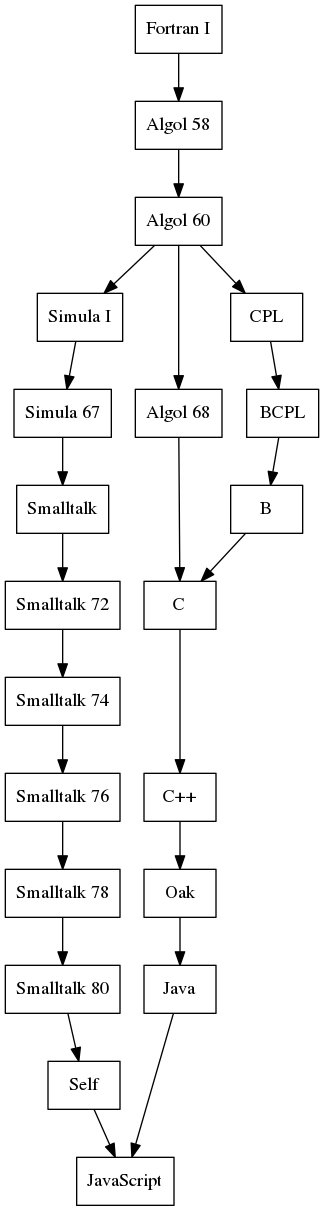
\includegraphics[height=0.5\textheight]{javascript}
  \captionof{figure}{Inheritance diagram for \cd{JavaScript}.}
\end{Figure}


\newpage
\end{document}
